\chapter{Introduction} % Main chapter title
\graphicspath{ {/Users/kaksonenlab/Desktop/figures/} }
\label{Ch:Intro} % Change X to a consecutive number; for referencing this chapter elsewhere, use \ref{ChapterX}

\section{Endocytosis and cell trafficking pathways}
The plasma membrane serves as the defining barrier between the interior and exterior of the cell, thus creating cellular identity, and facilitating evolution out of the primordial soup into a defined structure that can regulate entry of signals into the cell. In eukaryotes, and with increasing complexity, in multicellular eukaryotes, tuning cellular response to external signals has resulted in a complex network of signalling pathways, and tight coupling of these pathways with the process of endocytosis. Endocytosis refers to the uptake of molecules too big to simply pass through the plasma membrane. It involves the beinding of the plasma membrane into a cargo-filled invagination, and culminates in the severing of this invagination to form a vesicle. This vesicle and its contents are then targeted to other cellular organelles for either degradation or recycling. 


\vspace{5mm}

Apart from internalizing cargo, endocytosis allows regulation of the plasma membrane itself: its lipid and protein composition, and therefore many of its physical and biochemical properties like tension, rigidity, surface-receptor composition. Cargo taken up by endocytic pathways include these surface-receptors and their ligands that are transported across the cell, forming the link between cell signalling and endocytosis.
Endocytosis essentially forms the basis of all cellular responses, from incorporating external stimulus, to communication between different cellular compartments. This process arguably drove the development of organisms from single cell to multicellular eukaryotes.  
%	\includegraphics[width=21.5cm,height=21.5cm,keepaspectratio,



\vspace{5mm}
Plasma membrane regulation and internalization of signalling molecules are critical for the function of the cell. Among the vast array of important cargo that are taken up via endocytosis are cholesterol (Goldstein and Brown, 1973; Anderson, Goldstein and Brown, 1976), insulin (Fan et al., 1982), and other hormones. Not surprisingly, many human diseases have been linked to defects in the endocytic pathway like familial hypercholesterolemia- the study of which established the field of endocytosis, Alzheimer’s, and some types of cancer (Goldstein and Brown, 1973; Anderson, Goldstein and Brown, 1976, Maxfield, 2014, Mosesson, Mills and Yarden, 2008). The importance of the endocytic machinery as the entry portal into the cell is evident in the fact that it is hijacked by pathogens like viruses and bacteria to enter host cells (Mercer, Schelhaas and Helenius, 2010). Other components of the cellular signalling pathway transmit signals across the cell and between various organelles like the Golgi apparatus and endoplasmic reticulum. These membranes undergo similar transitions of the bounding membrane, and have mechanistic and biochemical similarities (McMahon and Mills, 2004; Traub, 2005), suggesting a universal principle of membrane deformation. 

\vspace{5mm}
Although many early discoveries relating to endocytic pathways were identified in mammalian cell types (Hemmaplardh and Morgan, 1976; Karin and Mintz, 1981), description of endocytosis in \textit{Saccharomyces cerevisiae} (Riezman, 1985) marked the beginning of the field of yeast endocytosis. Ease of genetic manipulation, availability of a completed genome sequence, and relative simplicity of endocytic pathways- there is only one- drove several discoveries that established yeast as a powerful model organism (Boettner, Chi and Lemmon, 2012; Payne, 2013).



\section{Clathrin-mediated endocytosis}
Many different endocytic pathways exist that facilitate the internalization of cargo at the plasma membrane, as depicted in Fig.\ref{intro_mayor}. These pathways select for differences in size and type of cargo. Of them, Clathrin-mediated endocytosis (CME), is universal among eukaryotes. In mammalian cells CME transports 90\% of labelled surface protein

\begin{figure}[H]
	%	\centering
	\hspace*{-1cm}
	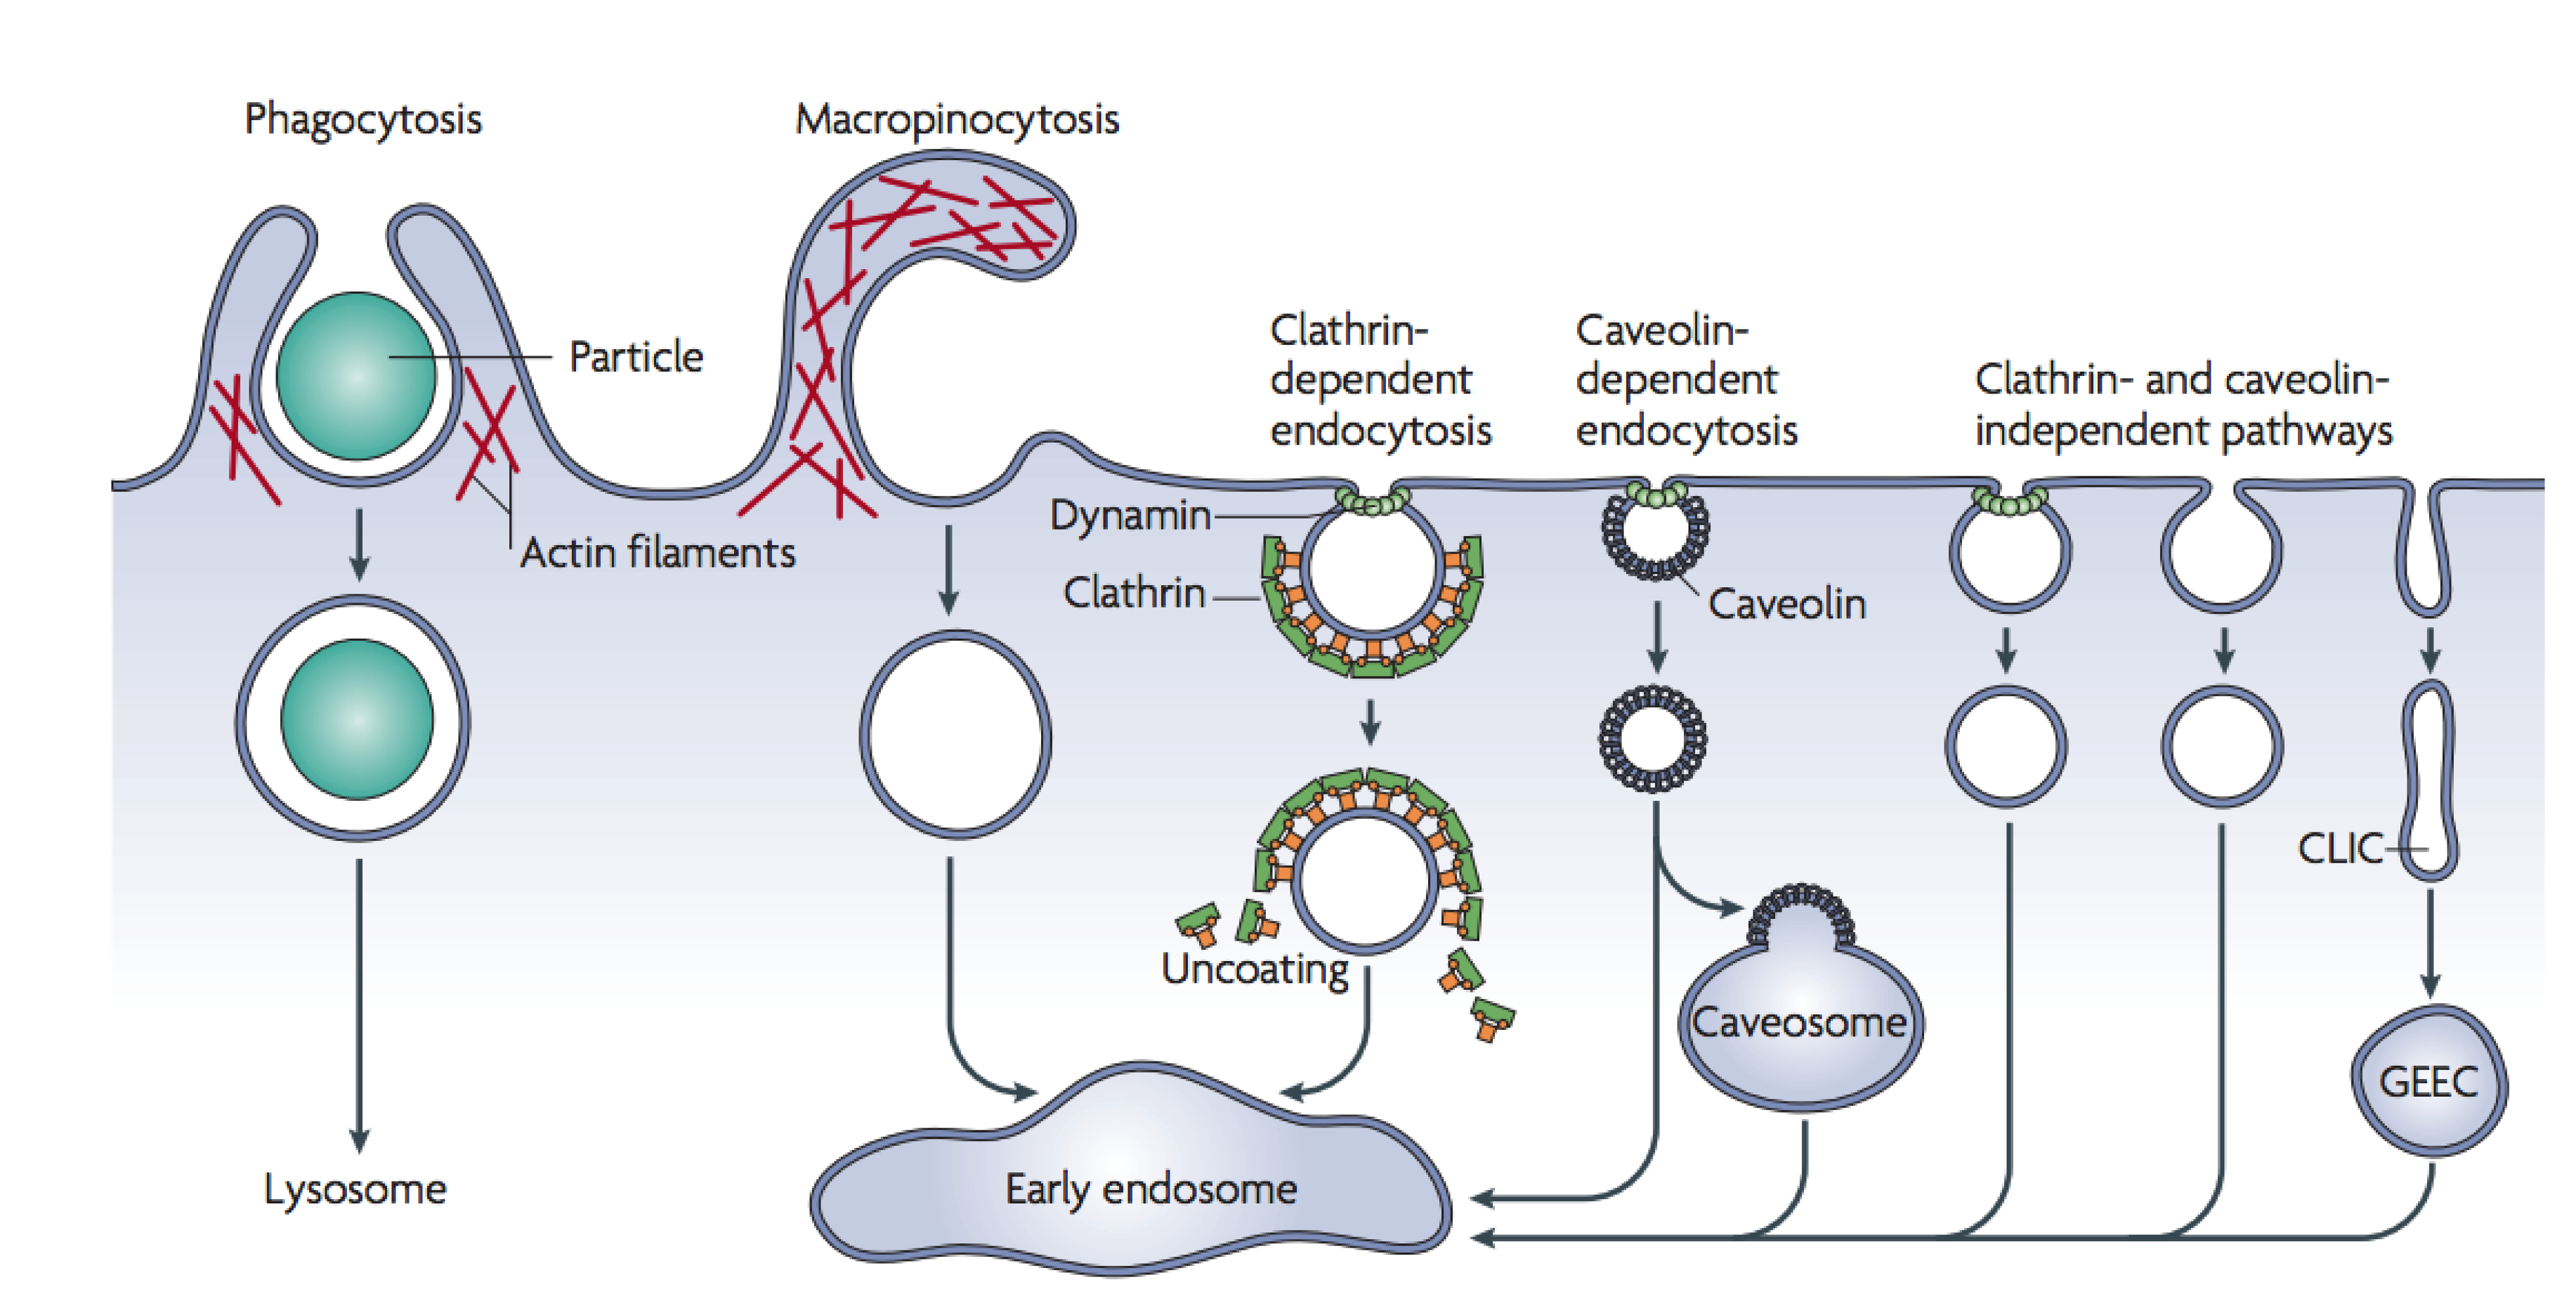
\includegraphics[width=14cm, height=16cm, keepaspectratio]{figures/intro/Fig1_mayor}
	\caption[Endocytic pathways in cells]
	{Some of the endocytic pathways in mammalian cells. Large particles are incorporated by phagocytosis, bulk fluid by macropinocytosis. A large array of cargo is taken into the cell via CME and calveolin-dependent endocytosis. Vesicles formed by these pathways are targeted to the early endosome. Clathrin and calveolin-independent pathways incorporate cargo and involve different geometries, including tubular "clathrin- and dynamin-independent carriers" (CLIC), that arrive at "GPI-anchored protein enriched early endosomes" (GEEC), before they are transported to endosomes.  \textit{Reprinted by permission from Springer Nature: Nature Reviews Molecular Cell Biology (Mayor and Pagano, 2007), copyright (2007)}
		\label{intro_mayor}}
\end{figure}

 into the cell (Bitsikas, Corrêa and Nichols, 2014). It was first identified when studying yolk uptake in mosquitos, and ultrastructural studies of their oocytes (where frequency of uptake events is high enough to be easily studied) identified a bristly coat formation inside the cell membrane and similarly bristly vesicles (Fig.\ref{intro_clathrin}). These vesicles then lost the bristly coat and fused to eventually form yolk bodies in the mature oocyte (Roth and Porter, 1964). The bristle was noted in several cell types, and later identified as a lattice of a single highly conserved protein (Pearse, 1976). This protein was named Clathrin, derived from the latin word for lattice. 


\vspace{5mm}
Clathrin is formed of light and heavy chains incorporated into a triskelion (Ungewickell and Branton, 1981) that assembles into closed hexagonal and pentagonal structures on the inner leaflet of the plasma membrane (Fig.\ref{intro_clathrin}). CME has, since four decades ago, been recognized has an ubiquitous mechanism of membrane uptake in cell types ranging from the frog presynaptic membrane (Heuser and Reese, 1973) to rat vas deferens (Friend and Farquhar, 1967). Clathrin also localizes to the trans-golgi network (TGN): these clathrin-coated vesicles mediate traffic from the TGN to the endosome. Specification of vesicle cargo and targeting to different cellular compartments is achieved by Clathrin interaction with specialized adaptor proteins like the adaptor protein complexes (AP), which specifies Golgi-to-early endosome traffic, while Golgi-localized gamma-adaptin (GGA) complexes specify Golgi-to-late endosome traffic (Payne, 2013). 



\begin{figure}[H]
	%	\centering
\hspace*{-0.6cm}
	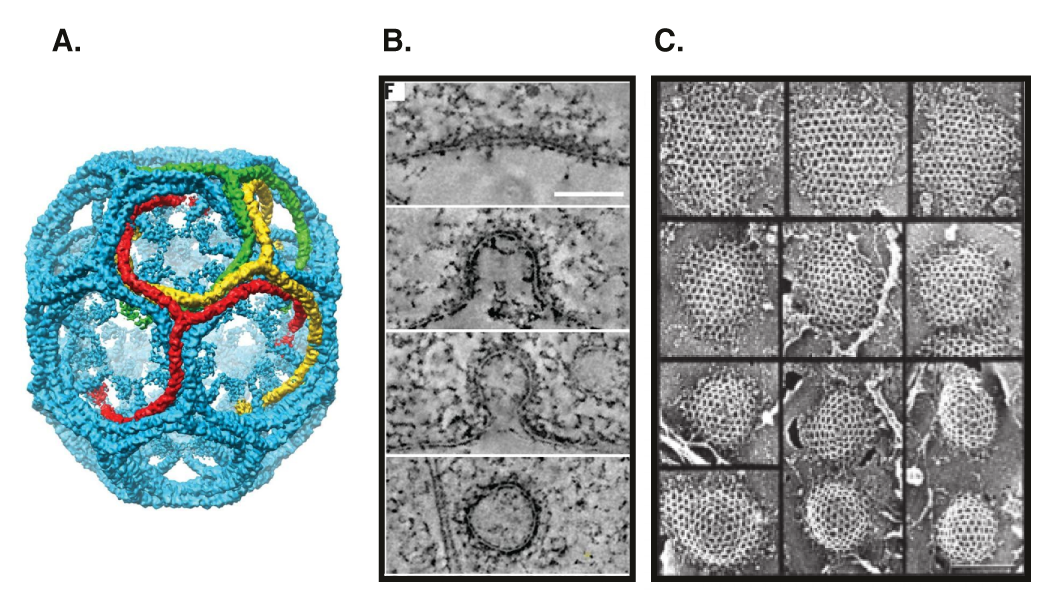
\includegraphics[width=14cm, height=17cm, keepaspectratio]{figures/intro/clathrin}
	\caption[Endocytic pathways in cells]
	{ A: Model for a clathrin-cated vesicle based on cryo electron microscopy.Three individual triskeleons are highlighted. \textit{Reprinted wjth permission from Springer Nature: Nature. Molecular model for a complete clathrin lattice from electron cryomicroscopy,  Fotin et al., Copyright 2004}.
		B:   Slices through tomograms of clathrin-coated pits in different stages of invagination. \textit{From Avinoam et al, Science 2016. Reprinted with permission from AAAS}
		C: Freeze-etch view of plasma membrane of mouse fibroblast showing a range of clathrin lattices. \textit{Republished with permission from CCC, from Three-dimensional visualization of coated vesicle formation in fibroblasts, Heuser, JCB 84, 1980 }
		\label{intro_clathrin}}
\end{figure}

	
\section{CME in mammalian and yeast cells }
		\subsection{Clathrin is required for mammalian CME}
The clathrin lattice was speculated as responsible for remodelling the plasma membrane and selecting cargo in the first papers that noted the “bristly” coat (Roth and Porter, 1964; Kanaseki and Kadota, 1969).  In multicellular organisms like \textit{Caenorhabditis elegans}, clathrin depleted by RNAi results in decreased endocytic uptake in oocytes and dead progeny (Grant and Hirsh, 1999). In \texit{Drosophila melanogaster}, deletion of clathrin heavy chain results in embryonic lethality (Bazinet et al., 1993). Knock-down of the heavy chain by RNAi in Hela cells results in decrease in endocytosis by 80\% (Huang et al., 2004). Essentially, endocytosis fails in the absence of clathrin in multicellular organisms. How exactly the clathrin coat shapes the progression of endocytosis has been heavily debated, but its involvement itself has not. 

\vspace{5mm}
Early work in yeast revealed that clathrin is not necessary for endocytosis (Payne and Schekman, 1985). Loss of clathrin only changes the size of the vesicles formed and leads to decrease in the number of established endocytic sites (Kaksonen, Toret and Drubin, 2005; Kukulski et al., 2016). Clathrin appears to affect establishment of sites and regulation of scission, but is not necessary for membrane invagination. It is now apparent that though the mammalian and yeast systems are mechanistically similar and most of the yeast endocytic proteins have mammalian homologues (Weinberg and Drubin, 2012), there are some significant differences.


		\subsection{Actin forces are required for yeast CME}
A single gene in yeast encodes the highly abundant actin protein, which is essential for cell survival (Koteliansky et al., 1979; Greer and Schekman, 1982). Organization of actin into axial filaments and cortical patches polarized to emerging buds was first described using phalloidin staining in fixed \textit{S. cervisiae} (Adams and Pringle, 1984). These patches were later established as dynamic endocytic sites by observing co-localization with other endocytic proteins (Kübler et al., 1993). While the mammalian CME is heavily dependent on clathrin for invagination, the yeast system relies on actin for endocytosis: disrupting actin filament formation blocks endocytosis (Kübler et al., 1993). 



	
		\subsection{CME in yeast is highly regular}
	In yeast, over fifty proteins are recruited, interact, and disassemble during the endocytic process. In mammals as well as in yeast, proteins that arrive at an endocytic site can be assigned into different modules according to their relative time of recruitment and function (Fig.\ref{intro_endpathway}). 

\vspace{5mm}
An initiation phase assembles coat proteins on the plasma membrane and establishes an endocytic site. The early proteins involved in the initiation phase are highly variable in both recruitment as well as time spent at sites. Initiation is followed by a very stereotypic sequence of events that assembles coat proteins, nucleates actin, organizes the actin network, invaginates a membrane tube, and finally severs the membrane to produce vesicles (Kaksonen, Toret and Drubin, 2005). While the entire process of initiation through scission occurs over a period of about a minute, once membrane invagination begins, inward movement and consecutive scission occurs in under fifteen seconds. This indicates tight regulation of the post-initiation sequence of events in the endocytic timeline. 

		\vspace{5mm}
Sterotypicity of the later stages of yeast endocytosis allows us to average the behaviour of a particular protein from multiple endocytic sites. Tracking the behaviour and organization of these proteins has led to a remarkably detailed understanding of the spatial and temporal regulation of endocytosis in yeast (Kaksonen, Toret and Drubin, 2005; Picco et al., 2015; Mund et al., 2017). The different stages of endocytosis are discussed below. 

		
 


			\subsubsection{Early initiation phase}
The initiation phase establishes endocytic sites and selects cargo (Brach et al., 2014). Deletion of an entire seven protein set of early endocytic proteins (Ede1, Syp1, Yap1801/1802, Apl1, Pal1, Pal2) does not prevent endocytosis. It seems that the initiation of endocytosis in yeast is independent of the recruitment of any one protein, and is likely a result of several different cooperative or independent factors (Brach et al., 2014). This could give the process robustness in the absence of alternate pathways for uptake of essential nutrients and signals. The variability in this phase could also provide a “check-point”, to ensure that sufficient cargo is loaded (Weinberg and Drubin, 2012) before later (energy consuming) phases are triggered. 


			
			\subsubsection{Coat module}
Coat proteins serve to template later-arriving proteins (Mund et al., 2017), as well as form the link between the actin network and membrane (Skruzny et al., 2012). Clathrin adaptors and the clathrin triskelion are not necessary for the progression of sites. Deletion of coat proteins Sla2 (Hip1R homologue) and Ent1 (Epsin homologue) results in what is known as an “uncoupling” phenotype. In these cells, actin polymerizes at the plasma membrane, but the membrane is decoupled from actin forces. This results in actin “flames” at cortical patches without membrane bending (Kaksonen, Sun and Drubin, 2003; Skruzny et al., 2012). A complex formed between Sla1, Pan1 and End3, which links the early coat to other coat proteins and polymerized actin, is involved in actin regulation itself, and connects vesicles to actin cables and endosomes (Wendland and Emr, 1998; Sun et al., 2015; Toshima et al., 2016). These proteins move inward into the cytoplasm with the membrane invagination
			



			\subsubsection{Actin module}
Once coat proteins are assembled, proteins that nucleate and organize a branched actin network are recruited. Actin filaments are nucleated by the Arp2/3 complex, acting in concert with actin nucleation promoting factors (NPFs): Wiscott-Aldrich syndrome protein (WASP) homologue Las17, type 1 myosins Myo3 and Myo5, intersectin homologue Pan1, and actin binding protein Abp1. Las17 is a potent actin nucleator, without which endocytosis essentially fails (Yidi Sun, 2006). Myo3/5 are non-processive motor proteins that interact with and can translocate actin filaments, but whose mechanistic contribution to endocytosis is unknown. Deletion of either Myo5 or Myo3 has subtle phenotypes, but deletion of both effectively blocked endocytosis (Yidi Sun, 2006). Abp1 binds actin filaments and is thought to activate the Arp2/3 complex. Without Abp1, cells are viable, but coat proteins persist on vesicles instead of disassembling after membrane scission. This suggests that Abp1 helps to dismantle the endocytic machinery. In support of this role, recruitment of late-stage enzymes like Ark1 and Prk1 that recycle endocytic proteins to membrane invaginations require Abp1. 


%\newpage



	\begin{figure}[H]
	\centering
	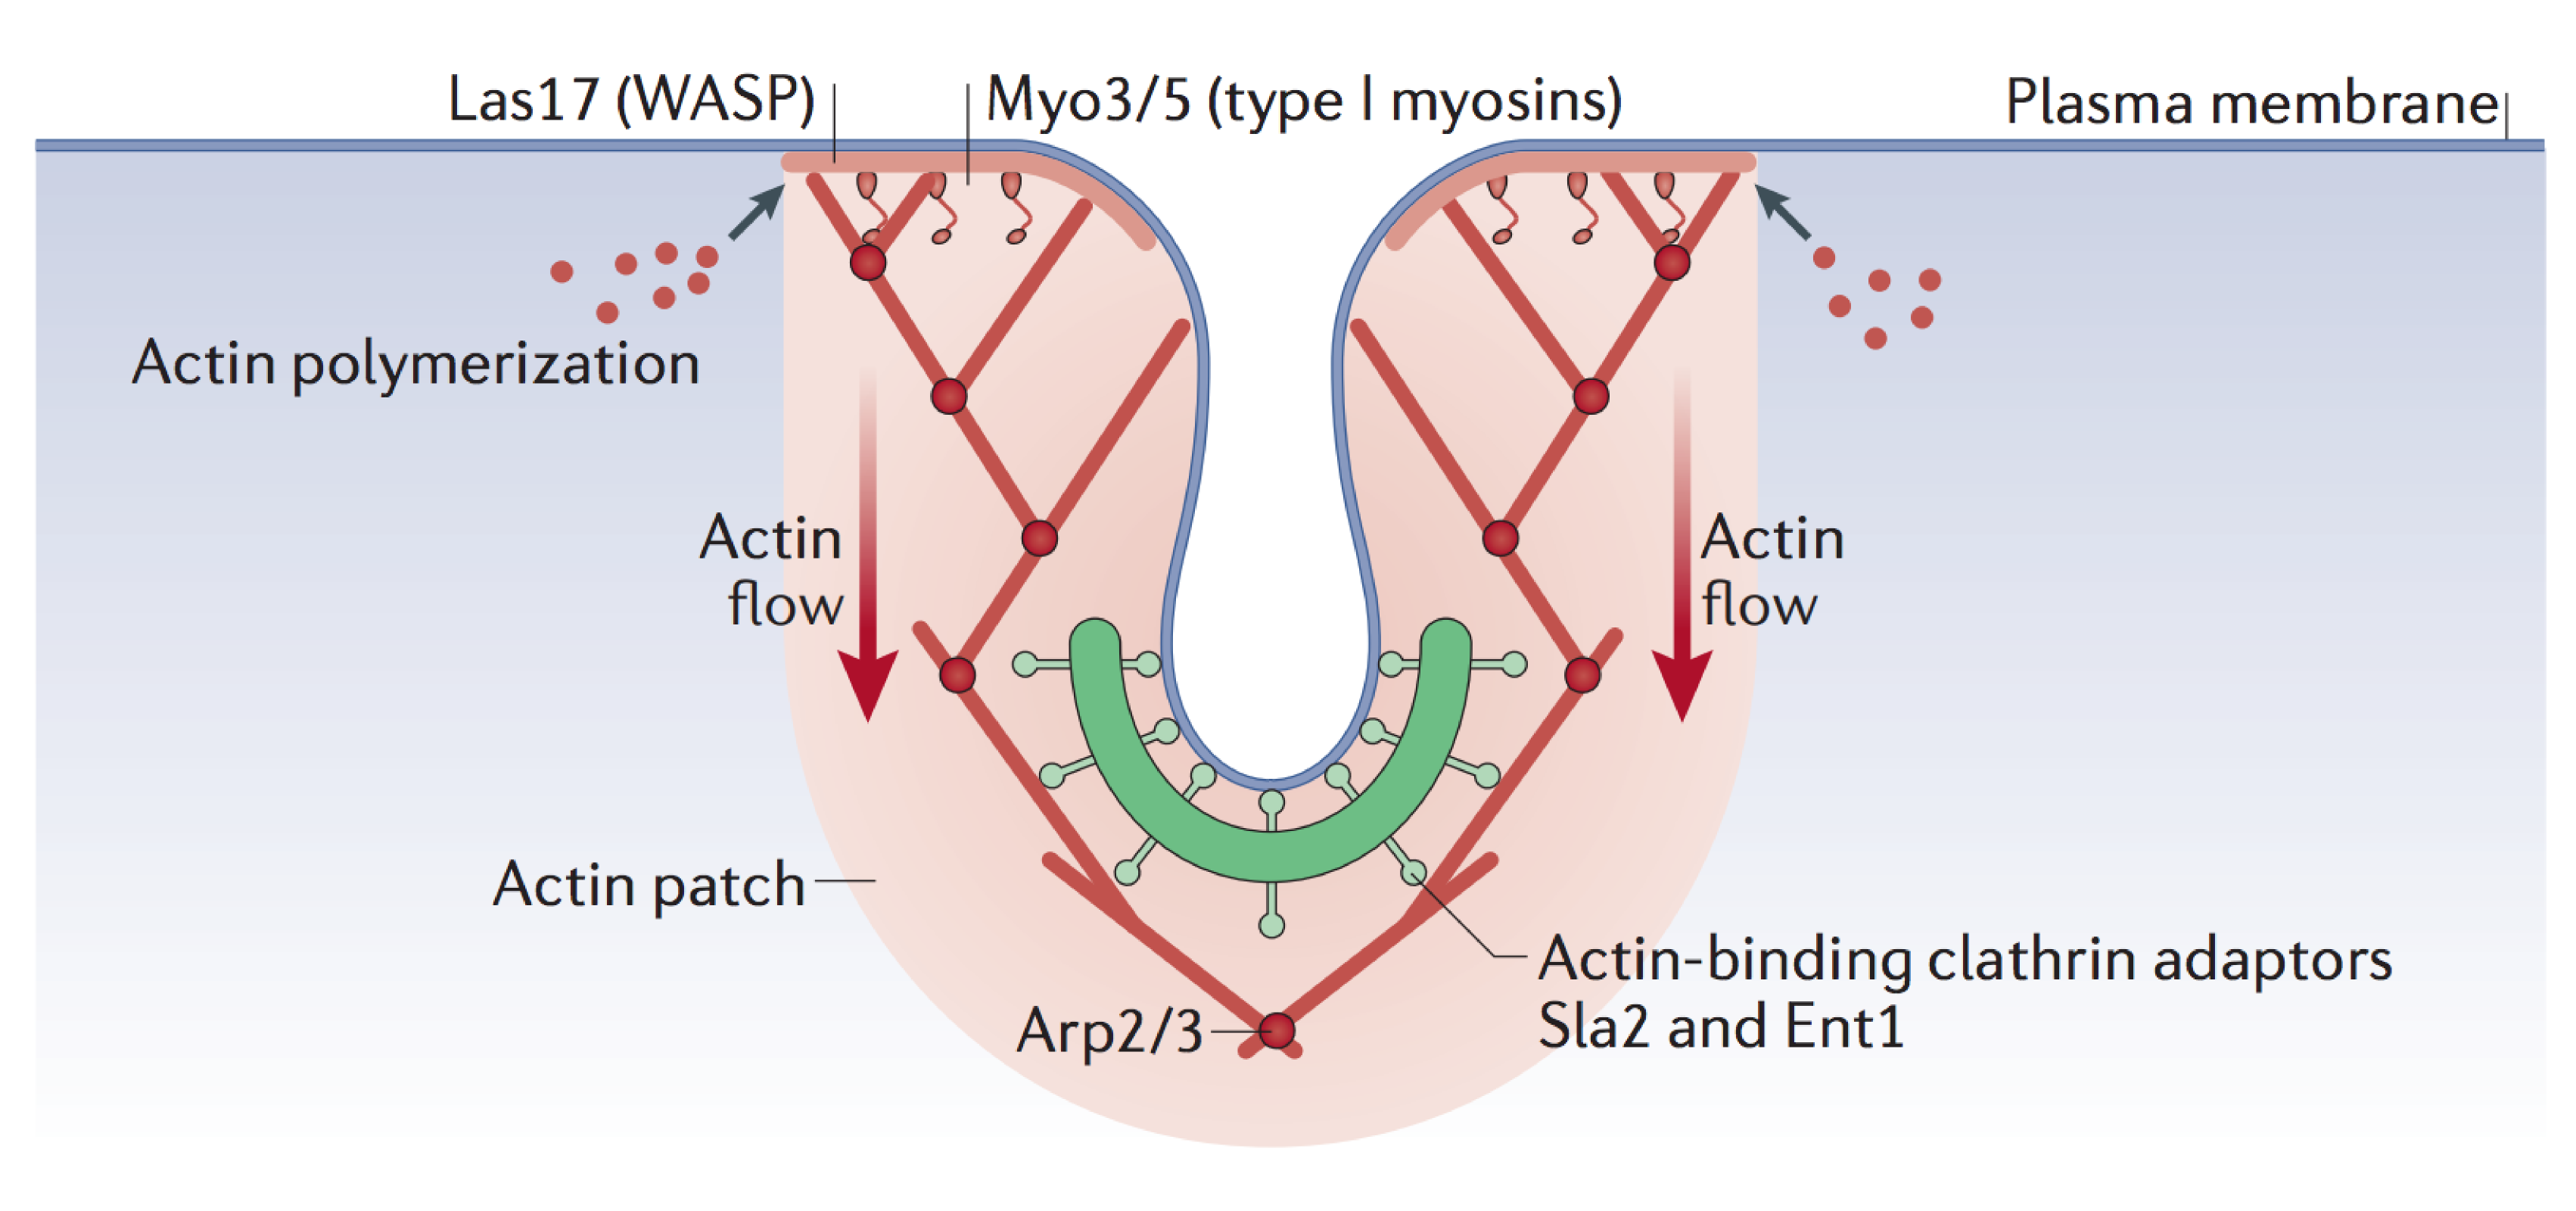
\includegraphics[scale=0.5]{figures/intro/actin_kaksonen}
	\caption[Actin network in endocytosis]
	{The model for actin-driven membrane invagination in yeast. Actin filaments are nucleated around the base of the invagination by the Arp2/3 complex, which is activated by Las17 and Myo3/5. Actin polymerization at the base pushes the actin network inward into the cell (actin flow). The actin network is coupled to the membrane by Sla2 and Ent1, which is also pulled inward with the actin network as actin filaments polymerize. \textit{Reprinted by permission from Springer Nature: Nature Reviews Molecular Cell Biology (Kaksonen and Roux, 2018), copyright (2018)
	\label{intro_actin_netork}}}
\end{figure}


%			\vspace{5mm}
Bbc1, Bzz1, and Vrp1 are other actin associated proteins that are recruited within the actin module. Bbc1 is known to inhibit Las17 NPF activity: its deletion accumulates actin at endocytic sites(Picco et al., 2018). Bzz1, an F-BAR protein, relieves Las17 of NPF activity inhibition by Sla1(Yidi Sun, 2006). Vrp1 acts in concert with myosins and Las17 to stimulate the Arp2/3 complex (Anderson et al., 1998; Wong et al., 2010). 

			\vspace{5mm}
Once NPFs and WASP/Myo proteins are recruited, Arp2/3 is recruited and actin polymerization begins. Actin crosslinkers like Sac6 and Scp1, capping protein complexes like Cap1/Cap2, Aip1/Cofilin, Abp1/Aim3 are recruited at this time. This begins the invagination of membrane. Actin monomers are added at the base of the invagination, and the actin network is linked to the membrane via coat proteins Sla2 and Ent1. As actin polymerization progresses, the entire actin network is pushed inwards, taking the membrane along with it (Picco et al., 2015).	

\newpage
\begin{figure}[H]
	\centering
	\hspace{-0.5cm}
	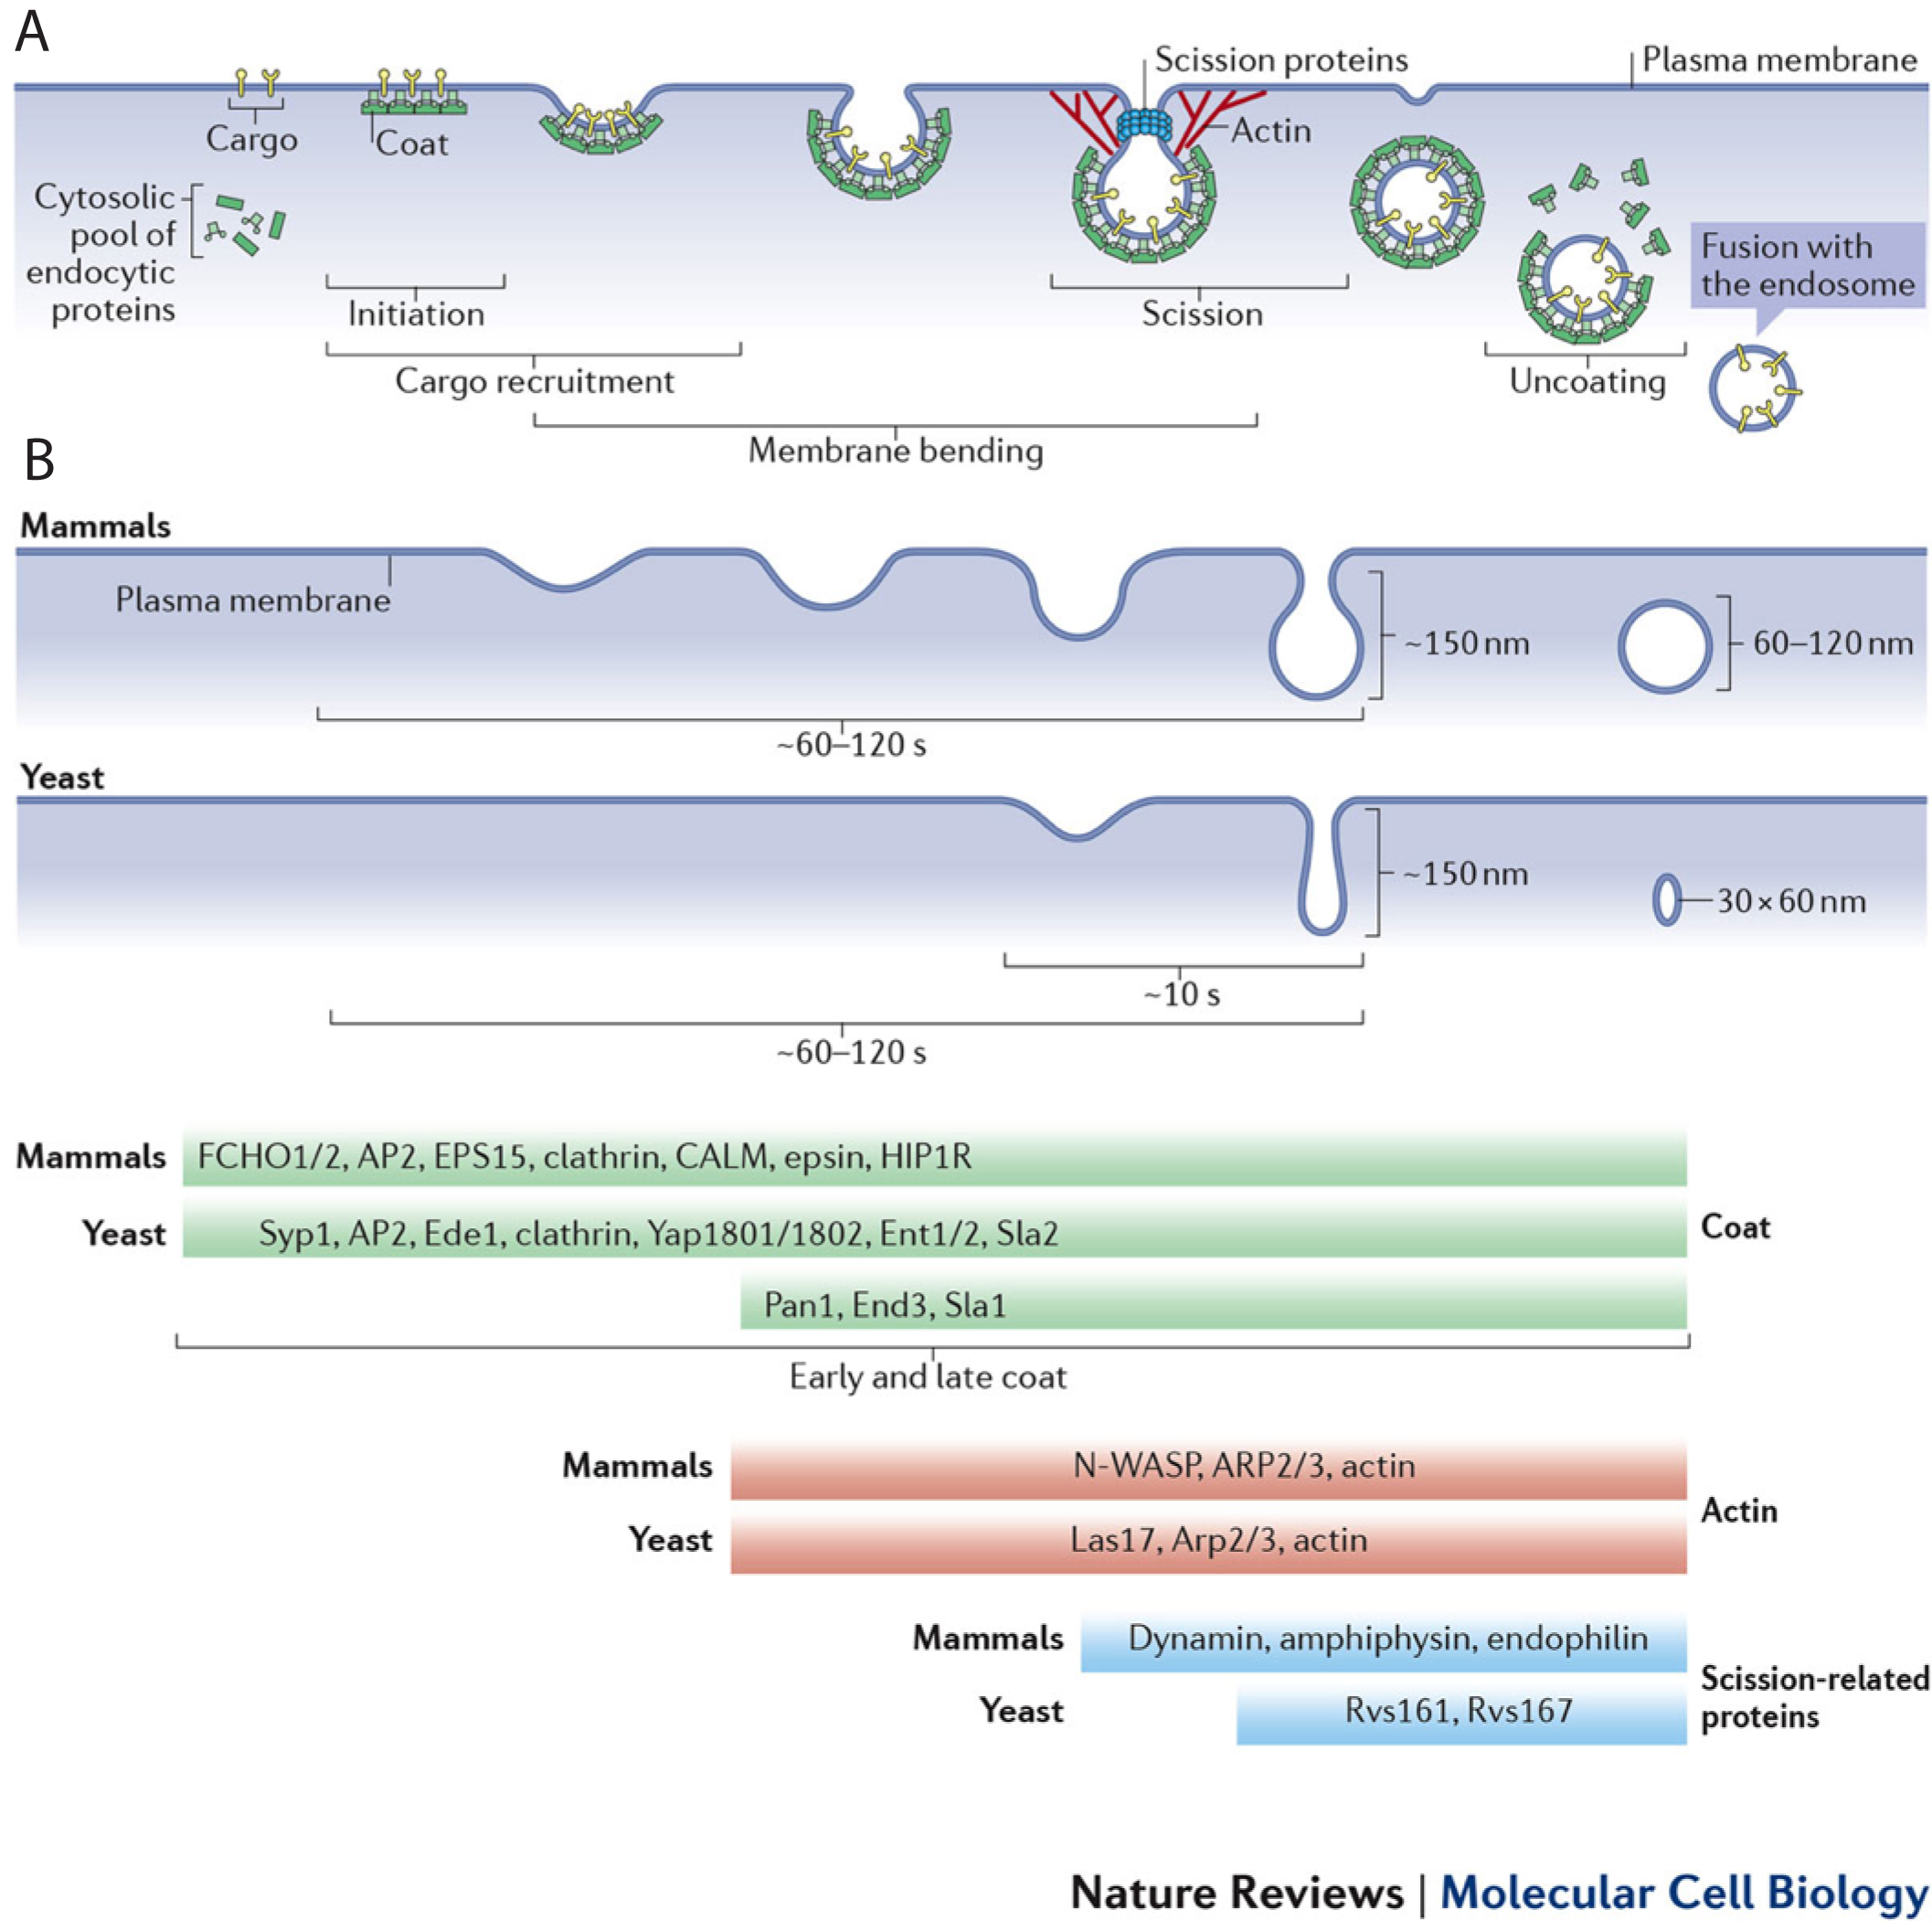
\includegraphics[scale=0.8]{figures/intro/Fig2_kaksonen}
	\caption[Endocytic pathway in mammalian and yeast cells]
	{A: Proteins involved in endocytosis are recruited from a cytoplasmic pool. Initiation of an endocytic event and cargo recruitment is followed by membrane bending. Membrane scission eventually forms a vesicle that releases its components, allowing it to be transported down the trafficking pathway. B: Membrane invagination in mammalian cells results in wider vesicles than in yeast cells. Proteins that are involved can be grouped based on their function in the endocytic pathway. Shown here are the main proteins involved, that are conserved between the two species. 
		\textit{Reprinted by permission from Springer Nature: Nature Reviews Molecular Cell Biology (Kaksonen and Roux, 2018), copyright (2018)}
		\label{intro_endpathway}}
\end{figure}

			\subsubsection{Scission module}
After the membrane invagination acquires a length of about 140nm, scission occurs, forming a vesicle. What actually causes scission in yeast is not yet determined (see /ref{yeastscission}).
The role of the dynamin in yeast endocytosis is unclear so far. N-BAR domain complex Rvs is recruited in the late stage of invagination, and membrane scission occurs shortly after it arrives (Kukulski et al., 2012; Picco et al., 2015). 
Coat proteins are finally disassembled from the vesicle after scission and the nascent vesicle is transported into the cell. Disassembly of coat components are regulated by kinases Ark1/Prk1 that phosphorylate several coat proteins like Sla1, Sla2, and Pan1. Glc17 and its adaptor Scd5 likely dephosphorylate these proteins so that can be incorporated into a new endocytic event. Yeast synaptojanins have also been implicated in late stages of the endocytic process, their contribution is discussed in . How the actin machinery is disassembled is not clear. Myosins and Las17 stop being recruited to sites seconds before scission occurs, so actin network disassembly is likely a result of increased rate of depolymerisation of actin filaments, compared to polymerization. 




		
		\newpage
\subsection{Membrane scission in mammalian cells}
		\subsubsection{Scission is dependent on dynamin} 
In mammalian cells, membrane scission in endocytosis is primarily effected by the GTPase dynamin. Dynamin was originally discovered as mediating interactions between microtubules (Shpetner and Vallee, 1989). It is now known to play a pivotal role in membrane scission and fusion events at many different cellular organelles. The importance of dynamin in endocytosis was demonstrated in a temperature sensitive mutant of the Drosophila shibire gene, which results in paralysis of flies at the non-permissive temperature. These flies fail to form synaptic vesicles (Grigliatti et al., 1973; Poodry and Edgar, 1979; van der Bliek and Meyerowrtz, 1991). Shibire codes for multiple isoforms of dynamin that are differentially expressed across the organism (Chen et al., 1991). Knock-down of dynamin isoforms disrupts vesicle-formation after invagination, resulting in accumulation of a large number of long membrane tubes (Ferguson et al., 2009). 

		\subsubsection{Dynamin is an oligomeric GTPase}
%		PIP\textsubscript{2}
Dynamins consist of a GTPase domain, a stalk region, a bundle signalling element that acts as the linker between the GTPase domain and stalk, a phosphatidylinositol (4,5)-bisphosphate (PtdIns(4,5)P2 , henceforth 	PIP\textsubscript{2})-binding pleckstrin homology domain (PH) domain and a proline rich domain (PRD) that extends beyond the GTPase domain (Antonny et al., 2016). \textit{In vitro}, dynamin oligomerizes into helical structures with the PH domain apposed against the membrane, and the GTPase domain facing away from the membrane (Sweitzer and Hinshaw, 1998; Zhang and Hinshaw, 2001). As depicted in Fig\ref{intro_dynamin_scission}, dynamin within the helical structure undergoes conformation changes upon GTP hydrolysis that constricts the helix as well as the membrane tube under it, collapsing the inner leaflet of the bilayer membrane into a hemi-fused state, resulting in membrane fission (Zhao et al., 2016). Disruption of its GTPase activity results in membrane tubes that accumulate dynamin and fail to undergo scission (Takei et al., 1995; David et al., 1996; Ringstad, Nemoto and De Camilli, 1997).

		
	\begin{figure}[H]
			\centering
			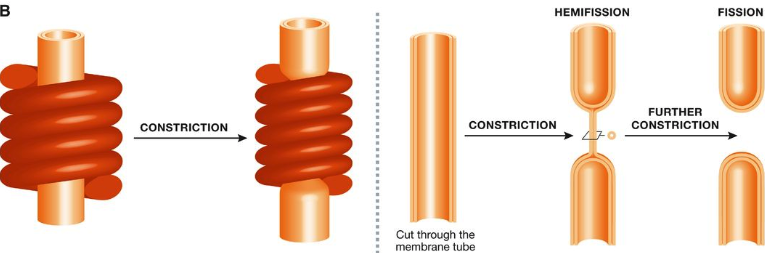
\includegraphics[scale=0.5]{figures/intro/dynamin_2}
\caption[Dynamin forms a scaffold]
					{some shit
					\textit{Reproduced from Antonny et al, under Creative Commons Cttribution Non-Commercial No Derivatives Licence CC BY-NC-ND}
		\label{intro_dynamin_scission}}
		\end{figure}


%(Adam et al., 2015) under creative commons licence \href{https://creativecommons.org/licenses/by/4.0/}{CC BY 4.0}}}

		\subsubsection{Dynamin interacts with BAR proteins to cause scission}
\textit{In vivo}, dynamin arrives at clathrin-coated pits via interaction with BAR proteins endophilin and amphiphysin (Ferguson et al., 2009). BAR domain proteins form intrinsically curved protein dimers named for the conserved module contained in their founding members, metazoan BIN/ Amphiphysin and yeast proteins Rvs167, Rvs161. In addition to the BAR domain, most BAR proteins have additional motifs that mediate their interaction with membranes or other proteins. Some BAR proteins have an N-terminal amphiphatic helix (N-helix) that is inserted into the membrane bilayer.  Others have phosphoinositide binding motifs like phox or pleckstrin homology (PH) domains, which direct BAR proteins to specific lipids within membranes. Some BAR proteins contain Src homology 3 (SH3) domains that mediate protein-protein interaction. These SH3 regions act as a scaffold for the proline-rich domains of dynamin (Grabs et al., 1997). 



		\subsubsection{Dynamin and BAR proteins interact via PRD and SH3 regions }
Dynamin’s PRD interacts with the SH3 domains of BAR proteins endophilin and amphiphysin (Grabs et al., 1997; Cestra et al., 1999; Farsad et al., 2001; Meinecke et al., 2013). Endophilin and dynamin appear to help recruit each other: Endophilin recruitment is reduced in the absence of dynamin, and vice-versa. Interaction with the endophilin BAR domain is also known to inhibit the GTPase action of dynamin (Farsad et al., 2001; Meinecke et al., 2013; Hohendahl et al., 2017). Meanwhile, amphiphysin levels are unchanged in absence of dynamin, while deletion of amphiphysin results in increased recruitment and prolonged lifetimes of dynamin and absence of membrane scission (Meinecke et al., 2013). These results suggest a role for amphiphysin for disassembly of dynamin involving GTP hydrolysis, and a role for endophilin in dynamin assembly. The mechanistic interplay between the two BAR proteins with dynamin is still debated, and the sequence of events that leads to membrane scission remains unclear (Neumann and Schmid, 2013; Hohendahl et al., 2017). Dynamin localization to clathrin-coated pits is not entirely dependent on BAR proteins, but both GTP hydrolysis and interaction with BAR proteins is necessary for efficient vesicle scission in mammalian cells (Shupliakov et al., 1997; Meinecke et al., 2013).


\label{key}

	\subsection{Membrane scission in yeast} \label {yeast_scission}
		\subsubsection{Yeast dynamin-like proteins}
In yeast, three dynamin-like large GTPases have been identified: Vps1, Dnm1, and Mgm1. Dnm1 and Mgm1 are involved in mitochondrial fission and fusion (Cerveny et al., 2007). Vps1 is essential for vacuolar protein sorting (Rothman et al., 1990), is involved in fission and fusion of vacuoles (Peters et al., 2004) and peroxisomes (Hoepfner et al., 2001), is required for regulation of golgi to endosomal trafficking (Gurunathan, David and Gerst, 2002). Vps1 may also arrive at early endocytic events(Nannapaneni et al., 2010). None of the three yeast dynamins have the typical PH domain (Bui et al., 2012; Moustaq et al., 2016) that in mammals interacts with the lipid bilayer. Instead, an “InsertB” region likely performs the same function. Although yeast dynamins also do not have PRDs that could interact with the SH3 domains of yeast BAR proteins, Vps1 has been shown to interact with clathrin and other endocytic proteins (Yu, 2004; Nannapaneni et al., 2010; Goud Gadila et al., 2017). Other work has failed to observe localization of Vps1 at endocytic sites (Kishimoto et al., 2011; Goud Gadila et al., 2017). The role of Vps1 in endocytosis is not clear, but it is a candidate for the role of the canonical dynamin in CME.



		\subsubsection{Yeast BAR domain proteins Rvs161/167 regulate scission timing}
In yeast, the Amphiphysin/ Endophilin homologue is the heterodimeric complex Rvs161/167 (Friesen et al., 2006) (Rvs). Apart from an N-BAR domain, Rvs167 has a C-terminal SH3 domain. Rvs arrives at endocytic sites in the last stage of the endocytosis, and disassembles rapidly at the time of membrane scission (Picco et al., 2015). Deletion of Rvs results in failure of membrane scission in nearly 30\% of endocytic events (Kaksonen, Toret and Drubin, 2005). Scission failure is identified by the movement inwards of the endocytic protein coat into the cytoplasm, followed by its retraction back towards the cell wall, indicating a failure to form vesicles. No mutation of other endocytic proteins exhibits this phenotype. Electron microscopy has shown that in \textit{rvs167\textDelta}  cells, vesicles formed are smaller than in wild-type (WT) cells. This profile suggests that although Rvs is not necessary for scission, localization of the complex makes scission more efficient, and influences the membrane length at which scission occurs. Some mutations like that of the yeast Syndapin Bzz1 and Synaptojanin Inp52 in the background of rvsΔ, exacerbates the retraction phenotype (Kishimoto et al., 2011), suggesting that Rvs might act in concert with other proteins. 

Forces that cause membrane invagination and scission
Forces are required to pull the membrane inwards, against turgor pressure, membrane rigidity, and membrane tension, that oppose deformation of the membrane. Estimates of these are in the order of 1000-5000pN (Dmitrieff and Nédélec, 2015), dominated by the high turgor pressure inside the yeast cells. Intracellular forces of this magnitude are typically provided by components of the cytoskeletal network like microtubules and actin filaments. Disrupting formation of actin filaments completely disassembles the actin network and stops endocytosis (Kübler and Riezman, 1993; Aghamohammadazadeh and Ayscough, 2009). A substantial amount of the force required to pull up the membrane therefore comes from actin polymerization.

Actin monomers polymerize into filaments at the base of endocytic invaginations (Picco et al., 2015). Polymerization of actin filaments against a membrane can generate forces that push away this membrane, a mechanism that is employed across many organisms and cell types to produce movement. For example, the bacteria Listeria propels itself across its host cell by high-jacking the actin machinery of the host, and polymerizing an actin “comet tail” behind it. 

Simulations show that the highest force requirement for membrane deformation occurs at the beginning of membrane invagination (Dmitrieff and Nédélec, 2015). After a tubular structure is formed, a constant force can continue to pull the tube into the cytoplasm. At the time of scission, rather than increasing the forces from actin, NPF activity has already plateaued (Picco et al., 2015). It is therefore not clear what causes the membrane tube to go from tube to vesicle.  

Rvs deletion appears to affect this transition, but its mechanistic contribution to this process has not been determined. Since yeast dynamins do not have PRDs, there is probably no interaction with Rvs. A mechanism that does not involve PRD-SH3 interactions like in mammalian cells is therefore likely. Several scission models have been presented in the literature so far. They are described briefly below and in more detail in the results section (see /ref{results}). 


%		\subsubsection{What causes scission?}
%		How Rvs may affect scission has not been determined. Since yeast dynamins do not have a PRD, there is likely no interaction with Rvs, so a mechanism that does not involve PRD-SH3 interactions like in mammalian cells is likely necessary. Yeast cells are under high turgor pressure that makes forces from actin polymerization necessary for invagination77,78. There is therefore likely to be some interplay between scission-stage proteins and the actin network that could modulate the final shape transitions. 

		
			\subparagraph{Proposed scission mechanisms}
			\mbox{}\\
			Although none of the three dynamin-like proteins has a proline-rich domain, increased membrane retractions have been seen in \textit{vps1\textDelta} \textit{rvs167\textDelta}  cells compared to \textit{rvs167\textDelta}  cells (Rooij et al., 2010), indicating that Vps1 might affect scission. 

			\vspace{5mm}
Another hypothesis has proposed that lipid hydrolysis by yeast synaptojanin-like proteins can cause vesicle scission (Liu et al., 2006). Synaptojanins dephosphorylate 	PIP\textsubscript{2}, a lipid subtype enriched at endocytic sites. In this model, Rvs would form a scaffold on the membrane tube, protecting the underlying 	PIP\textsubscript{2} . Hydrolysis of unprotected 	PIP\textsubscript{2} causes a boundary between hydrolyzed 	PIP\textsubscript{2} at the bud tip and BAR-covered 	PIP\textsubscript{2} at the tube. This lipid boundary produces a line tension at the interphase between the lipids that could generate enough force to pinch off a vesicle. 

%\textit{vps1\textDelta} \textit{rvs167\textDelta} 

			\vspace{5mm}
In-vitro experiments have suggested protein friction as a mechanism by which membrane scission could occur (Simunovic et al., 2017). In this model, a BAR domain scaffold exerts a frictional force on a membrane that is pulled under it. In-vivo, this pulling force could be generated by actin polymerization, while Rvs scaffolds the membrane tube. 
Recently, steric pressure exerted on the membrane by disordered protein domains that typically follow the BAR region has been proposed as a mechanism for scission (Snead et al., 2018). In these experiments, the amphiphysin BAR domain is able to drive scission, but scission efficiency increases three to four-fold because of the disordered protein regions. These regions do not need to have any specific biochemical properties: they can be replaced by any other disordered protein region. It has also been proposed that BAR domains scaffold membrane tubes and stabilize them, preventing scission (Boucrot et al., 2012; Dmitrieff and Nédélec, 2015). For a more detailed discussion on these models, see /ref{results}

			\vspace{5mm}
Many of these theories contradict each other, are based on \textit{in vitro} data, using mammalian BAR proteins, at protein concentrations orders of magnitude higher than physiological levels, and without the context of interaction partners, relevant membrane tension, native lipid composition and intra-cellular turgor pressure. Therefore, the mechanism for membrane scission in yeast is yet to be determined. 

 





		
\section{BAR domain proteins}
	
Proteins in the BAR protein superfamily have a BAR domain structure that is highly conserved across eukaryotes. BAR domain proteins are involved in a range of cellular processes including endocytosis, actin organization, cell polarity, transcription and tumor suppression (Sakamuro et al., 1996; Ren et al., 2006). 

Of the mammalian isoforms of the founding members, Bin1 (Amphiphysin II) and Bin3 are ubiquitously expressed, while Amphiphysin I is expressed only in neurons. The conserved portion of these proteins, as well as of Rvs167 and Rvs161, is an N-terminal region that forms the BAR domain. This domain typically forms dimers that have an intrinsic curvature defined by the dimerization angle. This curvature categorizes BAR proteins to classical BAR (high curvature), Fer–Cip4-homology-BAR (F-BAR, shallow curvature), and I-BAR (inverted curvature) (FigBARstructure). Membrane-binding is mediated by cationic clusters that bind via non-specific electrostatic interactions to anionic lipids like phosphatidyl serine (PS) or PIP\textsubscript{2}).

\vspace{2mm}

\begin{figure}[H]
	\centering
	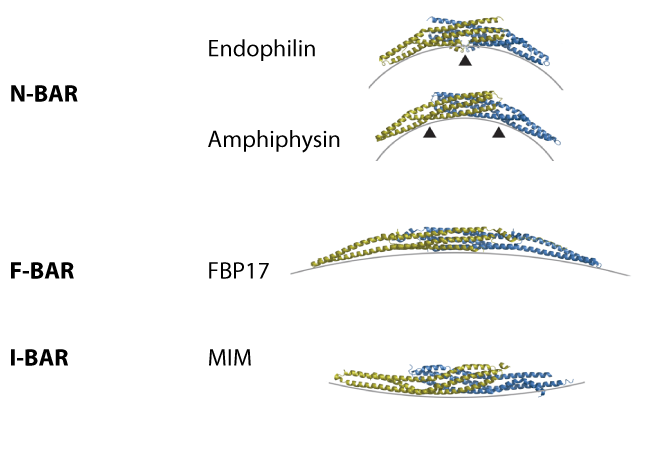
\includegraphics[scale=0.5]{figures/intro/BAR_structures}
		\caption[Structures of BAR domain dimers]{Domain structures from different families of BAR proteins. One monomer is depicted in yellow, the other in blue. Arrow heads indicate positions on the BAR domain that are inserted hydrophobically into the membrane. \textit{Adapted with persmission from John Wiley \& Sons, Inc.: The EMBO Journal (Qualmann, Koch, and Kessels, 2011), copyright (2011)}
		\label{bar_structures}}
\end{figure}

%\newpage
\vspace{5mm}
BAR dimers are able to oligomerize and scaffold large areas of membrane. These scaffolds can tubulate and generate curvature across membrane regions much larger than the dimensions of a BAR dimer(Farsad et al., 2001; Peter et al., 2004) (FigBARscaffold). BAR scaffolds can also bind membranes in a curvature-dependent manner. Correlation between the membrane shapes that they bind \textit{in vivo} and their intrinsic curvature has been shown for many BAR proteins. At membranes, they are thought to induce, stabilize, or generate specific curvature. 



		
\begin{figure}[H]
	\centering
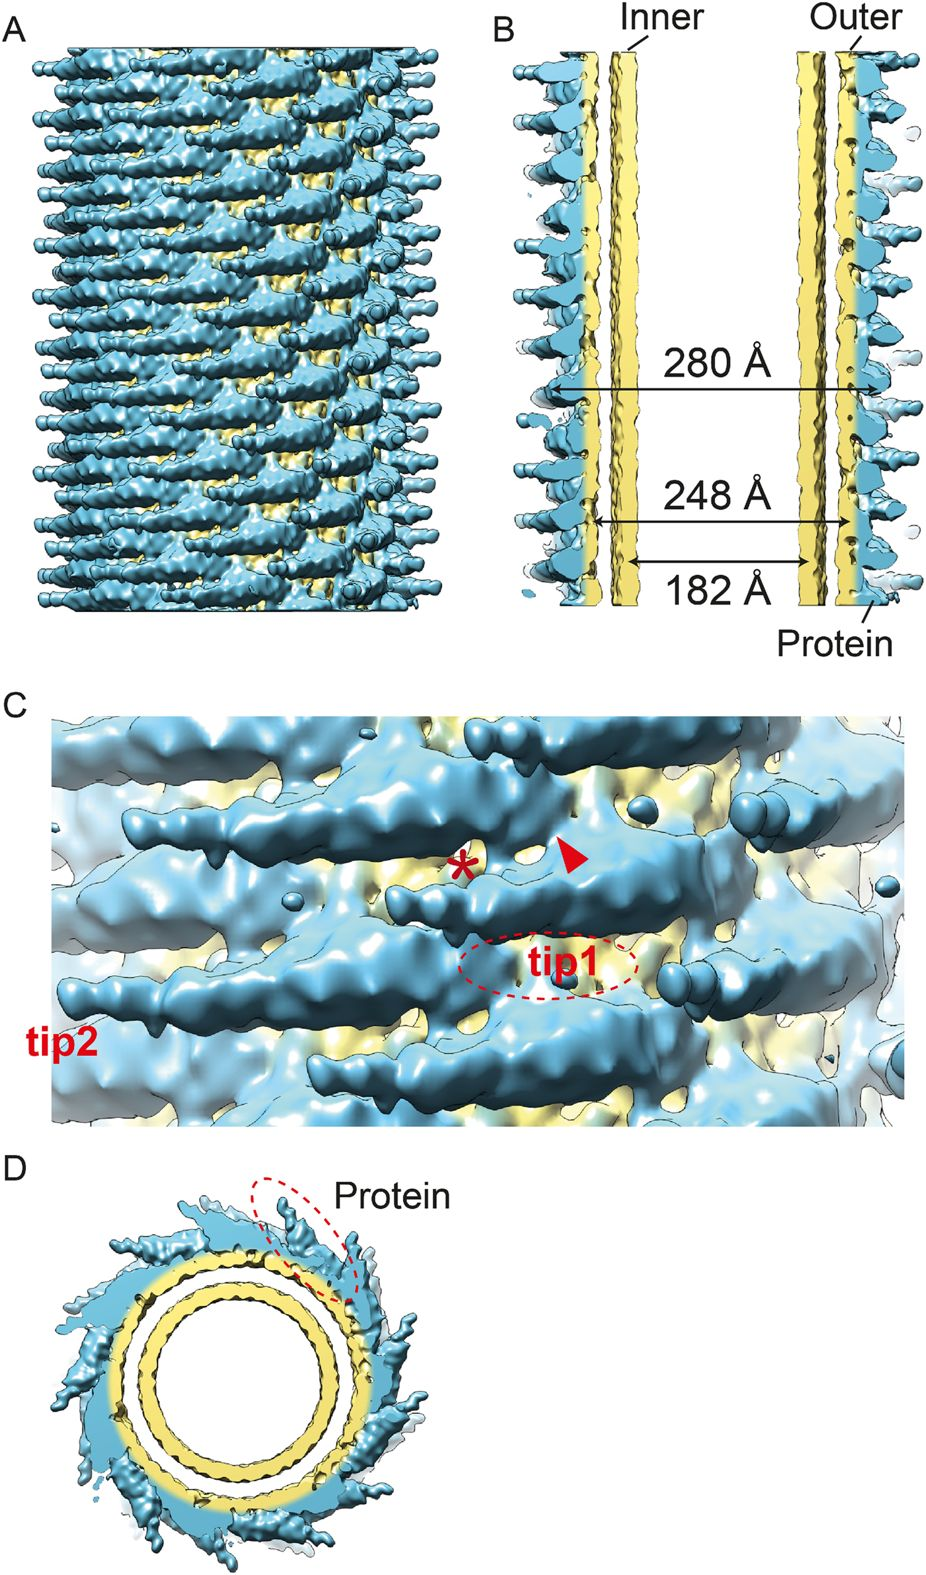
\includegraphics[scale=0.4]{figures/intro/BAR_scaffold}
\caption[BAR domain scaffolds]
{A: 3D reconstruction of amphiphysin-mediated tube from cryo-EM. Protein densities in blue,  lipid densities in yellow. B: Inner and outer leaflet of membrane is indicated. Numbers correspond to total diameter, and diameter of inner and outer membrane tubes. \textit{Figure reprinted from (Adam et al., 2015) under creative commons licence \href{https://creativecommons.org/licenses/by/4.0/}{CC BY 4.0}}
\label{intro_barscaffold}}
	\end{figure}



	\subsection{NBAR proteins and membrane shapes}	
Classical BAR domain proteins form a crescent-shaped structure. Some of them have an N-terminal amphiphatic helix (N-helix), forming a subclass of classical BAR called N-BAR domains. The two significant endocytic BAR proteins, Endophilins and Amphiphysins, are N-BAR proteins. 35-40 residues forms the N-helix that acts as an amphiphatic wedge that is unstructured until it is inserted into the membrane (Peter et al., 2004). The insertion causes displacement of lipids, resulting in bending of the membrane, indicating that N-helix insertion into a membrane bilayer could favour membrane scission (Kozlovsky and Kozlov, 2003; Boucrot et al., 2012). BAR domains lacking this helix are not able to efficiently tubulate  liposomes (Jennifer L Gallop, 2006). The N-helix also increases efficiency of binding to liposomes (Farsad et al., 2001) in a curvature sensitive manner, and confers salt sensitivity (Jennifer L Gallop, 2006). These experiments show that the N-helix likely interacts with membrane curvatures additionally to the BAR mechanism. 


	\vspace{5mm}
High resolution structural data has shown that N-BAR proteins can form helical scaffolds on tubular membranes (Peter et al., 2004; Shimada et al., 2007; Mim et al., 2012). An energetically favourable arrangement of BAR domains consists of dimers parallel to each other, apposed to the membrane. This scaffold favours membrane tubulation and prevents scission by stabilizing the membrane tube (Boucrot et al., 2012). N-helices combined with BAR scaffolds can therefore allow coexistence of both vesicles and tubules, with preference for one or the other depending on the ratio between number of N-helices that favour vesiculation, and BAR generated scaffold stability (Boucrot et al., 2012). 



	\vspace{5mm}
BAR proteins implicated in CME , Amphiphysin and Endophilin can tubulate membranes \textit{in vitro}(Peter et al., 2004; Jennifer L Gallop, 2006; Mim et al., 2012) and form a helical scaffolds via lateral interactions between BAR dimers (Sorre et al., 2012). 



	\subsection{NBAR protein in endocytosis: Amphiphysin }		
%		\subsubsection{Classical BAR domains : Amphiphysin}
Two mammalian isoforms of Amphiphysins (Amph) exist. AmphI is enriched in neurons in mammals, while AmphII (Bin1) is expressed in other tissue types, with one isoform enriched in muscle T-tubule junctions (Lee et al., 2002). The only Amphiphysin in flies (d-Amph) is expressed in various tissues, and enriched at muscle T-tubule junctions. The d-Amph dimer forms a coiled coil, with each BAR domain made of three long, kinked alpha-helices (Peter et al., 2004). In-vitro, liposome tubulation activity of Amphiphysin is concentration dependent. At very high concentrations, Amphiphysin is also able to sever tubular membrane to form vesicles (Peter et al., 2004). 

	\vspace{5mm}
Amph I and II both have BAR domains, a proline rich region, and C-terminal SH3 domain.
Amphiphysin I binds clathrin and its clathrin adaptor AP2 (Razzaq et al., 2001) and can polymerize clathrin into invaginated lattices in a BAR domain dependent manner(Peter et al., 2004). Both AmphI and AmphII also bind dynamin, and the lipid phosphatase Synaptojanin (Cestra et al., 1999).




	\subsection{NBAR protein in endocytosis: Endophilin }	
%		\subsubsection{Classical BAR domains : Endophilin}
The Endophilin A1-A3 (EndoA) family of genes were discovered in a screen for SH3 domain containing proteins (Giachino et al., 1997). EndophilinA were subsequently found to co-localize with dynamin, interact with Synaptojanin (Ringstad, Nemoto and De Camilli, 1997) and amphiphysin (Micheva et al., 1997): all three already identified as important regulators of synaptic vesicle recycling by endocytosis. A second mammalian protein was later discovered as related to endophilin, and termed EndophilinB (EndoB). 

	\vspace{5mm}
EndoA1 isoform is found in neurons, EndoA2 is expressed ubiquitously, and EndoA3 is enriched in the brain and testes. All three are found at presynaptic membranes. Crystal structure of EndoA1 shows the same overall structure as that of amphiphysin, with an additional amphiphatic helix similar to the N-helix, located at the centre of the crescent-shaped dimer (Weissenhorn, 2005; Jennifer L Gallop, 2006) (Fig,BARstructure). This helix is thought to insert into the membrane in the same way as the N- helix, potentially increasing membrane tubulation efficiency. EndoA1 and 2 may interact with calcium channels at synapses, and may be involved in lipid modification (Huttner and Schmidt, 2000; Gallop, Butler and McMahon, 2005), suggesting different roles for the two BAR domain proteins in membrane interaction. Endophilin interacts with dynamin, NWASP and Synaptojanin proteins via its SH3 domain (Cestra et al., 1999; Otsuki, Itoh and Takenawa, 2003; Hohendahl et al., 2017)





	\subsection{NBAR protein in yeast endocytosis: the Rvs complex}		
RVS167 and RVS161 (reduced viability upon starvation) genes were discovered in a screen that tested for survival under starvation conditions (Crouzet et al., 1991). Rvs167 and Rvs161 are both N-BAR domain proteins that are thought to form obligate heterodimeric complexes (Rvs) \textit{in vivo} (Sivadon, Crouzet and Aigle, 1997; Lombardi and Riezman, 2001). There is some evidence of heterodimerization: loss of one destabilizes the other, deletion phenotypes of Rvs167 is the same as that of Rvs161, and FCCS measurements indicate that they dimerize (Lombardi and Riezman, 2001; Kaksonen, Toret and Drubin, 2005; Boeke et al., 2014). However, Rvs161 functions that do not overlap with those of Rvs167 have been reported. Rvs161 for instance, interacts with Fus2 in cell-cell fusion, while Rvs167 does not (Brizzio, Gammie and Rose, 1998). It is likely that at endocytic sites the Rvs proteins function as heterodimers, while Rvs161 also forms heterodimers with Fus2. 

	\vspace{5mm}
Rvs161 and Rvs167 are similar in structure at the N-terminus, both contain N-BAR domains that are 42\% similar, 21\% identical, but are not interchangeable (Sivadon, Crouzet and Aigle, 1997). In addition to the BAR domain, Rvs167 has a Glycine-Proline-Alanine rich (GPA) region and a C-terminal SH3 region. The GPA region is thought to act as a linker with no known other function, while loss of the SH3 domain affects budding pattern and actin morphology. Most Rvs deletion phenotypes can however, be rescued by expression of the BAR domain alone ( Sivadon, Crouzet and Aigle, 1997), suggesting that the BAR domains are the main functional unit of the complex. Homology modelling has shown that the BAR domain of Rvs167 is similar to Amphiphysin and Endophilin (FigRvsstructure), and is therefore also likely to function similarly to the mammalian homologues. In keeping with this theory, Rvs has been shown to tubulate liposomes \textit{in vitro} (Youn et al., 2010). 


\vspace{5mm}
\begin{figure}[H]
	\centering
	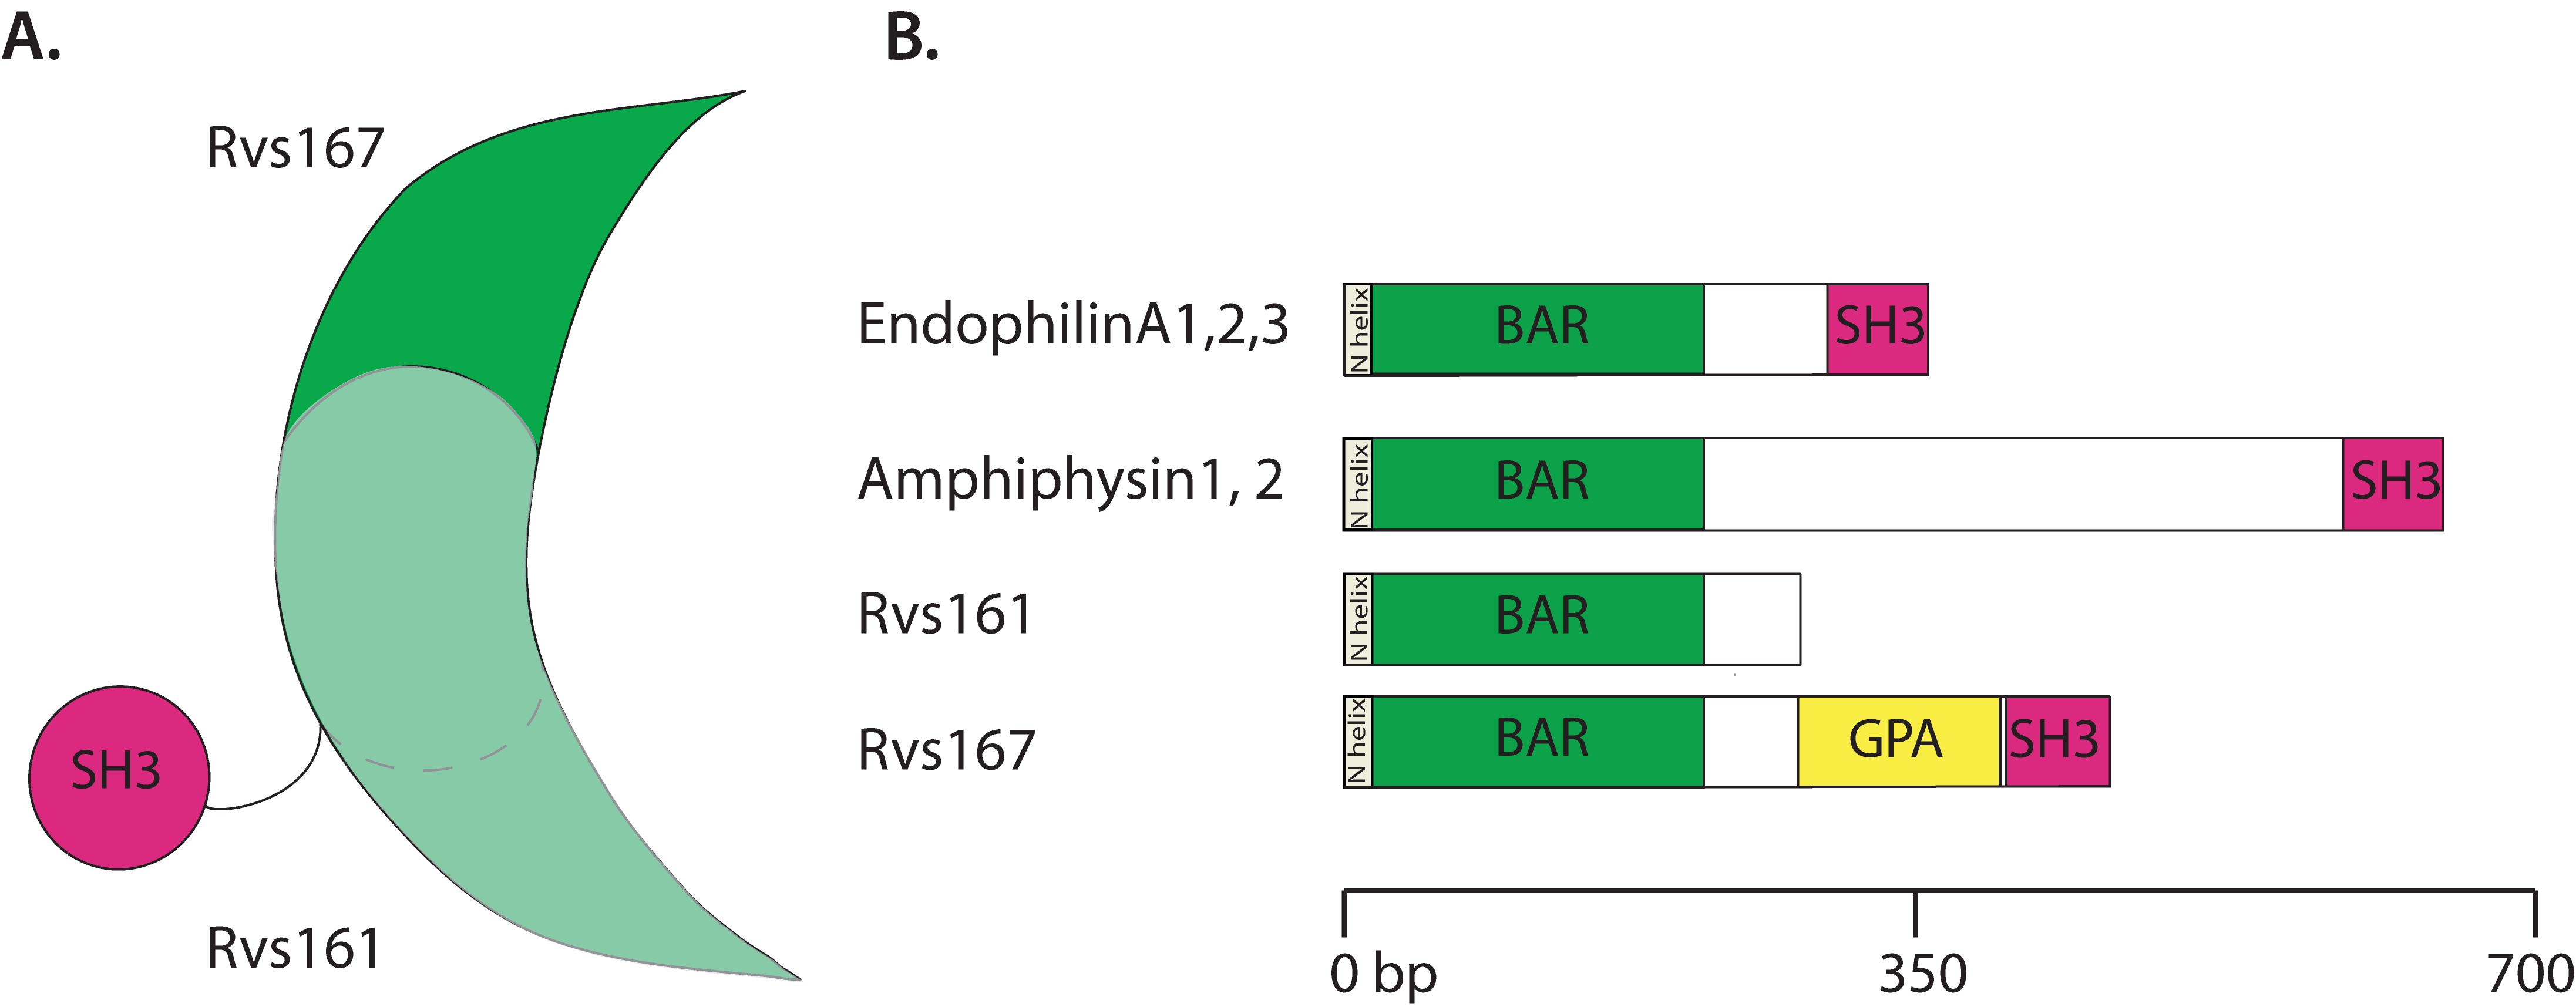
\includegraphics[scale=0.3]{figures/intro/Rvs_stucture2}
	\caption[Homolgy model of Rvs and BAR protein domains]
	{A: Cartoon of Rvs161 and Rvs167 BAR domain homology model based on d-Amph BAR domain structure. Rvs161 is shown in yellow and Rvs167 in cyan. 
		\textit{Reproduced from Youn et al, under Creative Commons Licence \href{https://creativecommons.org/licenses/by-nc-sa/3.0/}{CC BY-NC-SA 3.0}}
		B: domain structures of endocytic BAR domain proteins
		\label{rvs_structure}}
\end{figure}


	\vspace{5mm}
	\newpage
Cells with Rvs deleted cannot grow under high salt conditions. They are also sensitive to increased sphingolipid levels, and have random instead of bipolar budding pattern (Bauer et al., 1993; Sivadon et al., 1995; Lombardi and Riezman, 2001; Toume and Tani, 2016). Rvs deleted cells also have aberrations in actin localization: instead of actin patches polarized to emerging buds, patches are homogenously distributed across mother and daughter cells. Loss of Rvs therefore affects localization of actin, and heightens sensitivity of yeast cells to stressful growth conditions.
 	
 	\vspace{2mm}
Rvs arrives at endocytic sites has shown that Rvs arrives in the last stage of endocytosis (Kaksonen, Toret and Drubin, 2005; Picco et al., 2015). When maximum number of Rvs is recruited, that is, at peak fluorescent intensity, movement of the Rvs complex shows a jump inwards into the cytoplasm, concomitant with a sharp decay in its fluorescent intensity, a behaviour unique among endocytic proteins (Kaksonen, Toret and Drubin, 2005; Picco et al., 2015). As mentioned earlier, loss of Rvs also affects membrane scission efficiency and causes formation of smaller vesicles than in wild-type (WT) cells. How the Rvs complex affects membrane scission, and what eventually causes membrane scission are the major questions addressed in this work




		

%(Adam et al., 2015) under creative commons licence \href{https://creativecommons.org/licenses/by/4.0/}{CC BY 4.0}}}
%\begin{itemize}
%	\item Is localization microscopy suitable to study endocytosis in budding yeast?
%\end{itemize}
